\documentclass[11pt]{beamer}
% Compile with pdfLaTeX.

\usetheme{Boadilla}


\definecolor{SBred}{RGB}{153,0,0}
\definecolor{AttentionBlue}{RGB}{35,95,170}


\definecolor{SBred}{RGB}{153,0,0}
\definecolor{Ink}{RGB}{38,38,38}
\definecolor{Muted}{RGB}{105,105,105}

\makeatletter
\colorlet{beamer@blendedblue}{SBred}
\makeatother

\setbeamercolor{normal text}{fg=Ink,bg=white}
\setbeamercolor{frametitle}{fg=SBred,bg=white}
\setbeamercolor{structure}{fg=SBred}

% White footer text.
\setbeamercolor{author in head/foot}{fg=white,bg=SBred}
\setbeamercolor{title in head/foot}{fg=white,bg=SBred!70!white}
\setbeamercolor{date in head/foot}{fg=white,bg=SBred!45!white}

\setbeamerfont{frametitle}{size=\large}
\setbeamertemplate{navigation symbols}{}
\setbeamertemplate{page number in head/foot}[totalframenumber]
\setbeamersize{text margin left=7mm,text margin right=7mm}

\usepackage[T1]{fontenc}
\usepackage{lmodern,amsmath,amssymb,mathtools,booktabs,array,graphicx}
\usepackage{tikz}
\usetikzlibrary{positioning,arrows.meta,calc}

\hypersetup{
  colorlinks=true,
  urlcolor=SBred,
  pdftitle={Attention Factors for Statistical Arbitrage: Final report},
  pdfauthor={Jiaxi Cao}
}

\newcommand{\learn}[1]{\textcolor{SBred}{#1}}
\newcommand{\src}[1]{%
  \par\vfill
  {\fontsize{6.4}{7.6}\selectfont\color{Muted}#1\par}
}
\newcommand{\claim}[1]{%
  \par{\color{SBred}\bfseries #1\par}
}
\newcommand{\R}{\mathbb R}
\newcommand{\Var}{\operatorname{Var}}

\newcommand{\sbulogo}{%
  \IfFileExists{assets/sbu_logo.png}
    {
\includegraphics[width=22mm]{assets/sbu_logo.png}}
    {\textcolor{SBred}{\scriptsize Stony Brook University}}
}

% SBU logo at the upper right of each titled frame.
\setbeamertemplate{frametitle}{%
  \vspace{2mm}
  \begin{minipage}[c]{.75\textwidth}
    \raggedright\insertframetitle
  \end{minipage}\hfill
  \begin{minipage}[c]{.22\textwidth}
    \raggedleft\sbulogo
  \end{minipage}
  \vspace{2mm}
}

\title[Attention Factors]{%
  \textbf{Attention Factors for\\Statistical Arbitrage}
}
\subtitle{Final report: model, data and results}
\author[Jiaxi Cao]{Jiaxi Cao}
\institute[Stony Brook]{Stony Brook University}
\date[AMS 520]{%
  AMS 520: Machine Learning in Quantitative Finance\\Fall 2026
}

% Display the short title as plain text, without an internal link.
\makeatletter
\renewcommand{\insertshorttitle}[1][]{\beamer@shorttitle}
\makeatother

\newcommand{\threequestions}{%
  \[
  \boxed{\begin{array}{ccccc}
    \substack{\text{Which stocks}\\\text{are similar?}}
    &\longrightarrow&
    \substack{\text{What counts}\\\text{as mispricing?}}
    &\longrightarrow&
    \substack{\text{How to}\\\text{trade it?}}
  \end{array}}
  \]
}

\newcommand{\strategyroadmap}{%
  \[
  \boxed{\begin{array}{ccccc}
    \substack{\text{Which stocks}\\\text{are similar?}}
    &\longrightarrow&
    \substack{\text{What counts}\\\text{as mispricing?}}
    &\longrightarrow&
    \substack{\text{How to}\\\text{trade it?}}\\[4mm]
    \textcolor{SBred}{\text{Attention}}
    &&
    \textcolor{SBred}{\text{LongConv}}
    &&
    \textcolor{SBred}{\text{Net Sharpe + Explained Var.}}
  \end{array}}
  \]
}

% ---------------------------------------------------------------------------
% Final report deck, in the style of the Phase I deck (slides/Phase1/main.tex).
% Everything above is that file's preamble, unchanged apart from \subtitle and
% pdftitle, so a Phase I frame pasted below compiles as it is. Copy any figure
% it uses from Phase1/assets/ into assets/.
%
% Conventions of the Phase I deck:
%   \claim{...}       the frame's takeaway: one bold line in SBU red
%   \learn{...}       learned parameters, red inside equations (never a function's name)
%   \src{...}         small source line at the bottom of a frame (grey in Phase I)
%   \threequestions, \strategyroadmap
%                     the boxed three-step roadmap; a section divider repeats
%                     the box with the current step in \textbf
%   AttentionBlue     second accent, for a contrast with SBred
%   \note{...}        last in a frame: "45 seconds." and then the spoken text
%   figures           assets/<name>.png, with
%                     [width=\linewidth,height=4.0cm,keepaspectratio], \caption
%   tables            booktabs with @{} at both ends; \small, or
%                     \fontsize{6.4}{7.4}\selectfont for a dense table
%   order             title, main slides, References, Thanks!, backup slides
% ---------------------------------------------------------------------------

% Title pages (the user's requests, 2026-11-15). Sections 2 to 6 open with \sectiontitlepage, and every
% subsection opens with one too. The section's name is large and bold, at the same place on every title
% page; a subsection's name is set below it in smaller type. \secname and \subsecname are plain text
% (\insertsectionhead is a link and would take the link colour).
\newcommand{\titlepageframe}[1]{%
  \begin{frame}{\phantom{Section}}
  \vfill
  \centering
  {\color{SBred}\LARGE\bfseries\secname\par}
  \medskip
  {\color{SBred}\large#1\par}
  \vfill\vfill
  \end{frame}
}
\newcommand{\sectiontitlepage}{\titlepageframe{\strut}}
\AtBeginSubsection[]{\titlepageframe{\subsecname}}

% Two departures from Phase I (the user's instructions, 2026-11-15):
%   no grey text: \src and figure labels are in the text colour;
%   no roadmap box between parts: slide 2 is a table of contents of the \section titles.
\renewcommand{\src}[1]{%
  \par\vfill
  {\fontsize{6.4}{7.6}\selectfont#1\par}
}
% Links, such as the entries of the contents slide, in SBU red like the frame titles
% (hyperref's default link colour is a brighter red).
\hypersetup{linkcolor=SBred}

\begin{document}
\begin{frame}{\phantom{Attention Factors for Statistical Arbitrage}}
\vspace{-4mm}\titlepage
\vspace{-5mm}
\begin{center}\scriptsize Based on Epstein, Wang, Choi and Pelger (ICAIF 2025)\\
\href{https://doi.org/10.1145/3768292.3770398}{doi:10.1145/3768292.3770398}\end{center}
\end{frame}

% --- Main slides ------------------------------------------------------------

\begin{frame}{Contents}
\tableofcontents
\end{frame}

\begin{frame}{Recap: The Paper's Roadmap}
\claim{Train the comparison portfolios and trading policy together.}
\strategyroadmap
Phase I explained this model. Today we build it, feed it our own data and test it.
\end{frame}

% ============================================================================
\section{Building the model}

\begin{frame}{The Model in Four Steps}
\small
\setlength{\abovedisplayskip}{2pt}
\setlength{\belowdisplayskip}{3pt}

\claim{1. Attention builds $K$ factor baskets from the characteristics}\par
\[
A_{t-1}=\operatorname{softmax}_{\text{stocks}}\!\left(
\frac{\learn{Q}\,(X_{t-1}\learn{W})^{\mathsf T}}{\sqrt d}\right),
\qquad
F_t=A_{t-1}R_t.
\]

\claim{2. Ridge loadings turn the baskets into residual portfolios}\par
\[
\beta_{t-1}^{\mathsf T}
=A_{t-1}^{\mathsf T}\!\left(A_{t-1}A_{t-1}^{\mathsf T}+\lambda_{\rm ridge}I_K\right)^{-1},
\qquad
\epsilon_t=\underbrace{\left(I_N-\beta_{t-1}^{\mathsf T}A_{t-1}\right)}_{P_{t-1}}R_t.
\]

\claim{3. LongConv reads 30 past residuals and sets a position}\par
\[
s_{i,t-1}=\operatorname{LongConv}_{\learn{\theta}}
\left(\epsilon_{i,t-30},\ldots,\epsilon_{i,t-1}\right).
\]

\claim{4. Positions go back to stocks, with total absolute exposure one}\par
\[
\omega_{t-1}
=\frac{P_{t-1}^{\mathsf T}s_{t-1}}{\|P_{t-1}^{\mathsf T}s_{t-1}\|_1}.
\]
\end{frame}

\begin{frame}{LongConv: The Block We Built}
\small
\setlength{\abovedisplayskip}{2pt}
\setlength{\belowdisplayskip}{3pt}
The paper gives the convolution. The layers around it are our choice.

\smallskip
\claim{1. Encode each day's residual, in percent, into 32 channels}\par
\[
u_{i,h,\tau}=\learn{a_h}\,(100\,\epsilon_{i,t-30+\tau})+\learn{b_h},
\qquad h=1,\ldots,32,\quad\tau=0,\ldots,29.
\]

\claim{2. Filter each channel through time, as in Phase I}\par
\[
y_{i,h}
=\sum_{\ell=0}^{29}\learn{\overline{\mathcal K}_{h,\ell}}\,u_{i,h,29-\ell}
+\learn{D_h}\,u_{i,h,29}.
\]

\claim{3. Mix the channels, and keep a shortcut to yesterday's residual}\par
\[
z_i=\operatorname{LayerNorm}_{\learn{\gamma}}\!\Big(u_{i,\cdot,29}
+\operatorname{Linear}_{\learn{\psi}}\big(\operatorname{Dropout}(\operatorname{GELU}(y_{i,\cdot}))\big)\Big).
\]

\claim{4. Read out one signed position}\par
\[
s_{i,t-1}=\learn{v}^{\mathsf T}z_i+\learn{b_s}.
\]
\end{frame}

\begin{frame}{The Objective We Train: Annualized Net Sharpe}
\small
On each batch of 126 consecutive trading days, with $\overline n$ and $\sigma(n)$ the mean and
standard deviation of $n_t$:
\[
\max_{\learn{W},\,\learn{Q},\,\learn{\theta}}
\left[
\underbrace{\sqrt{252}\;\frac{\overline n}{\sigma(n)}}
            _{\text{annualized net Sharpe}}
+\lambda_{\rm Var}
\underbrace{
\frac1N\sum_{i=1}^{N}
\left(
1-\frac{\Var_t(\epsilon_{i,t})}{\Var_t(R_{i,t})}
\right)
}_{\text{explained variance}}
\right],
\qquad\lambda_{\rm Var}=100.
\]
\[
n_t=\underbrace{(R_t-R_{f,t})^{\mathsf T}\omega_{t-1}}_{\text{gross excess return}}
-\underbrace{0.0005\,\|\omega_{t-1}-\omega_{t-2}\|_1}_{5\ \mathrm{bp}\ \text{per traded unit}}
-\underbrace{0.0001\sum_j(-\omega_{j,t-1})_+}_{1\ \mathrm{bp}\ \text{on short exposure}}.
\]
The risk-free rate $R_{f,t}$ is subtracted from every stock's return first, so $n_t$ is an excess
return: the book pays $R_f$ on its net position $\sum_j\omega_{j,t-1}$.
\end{frame}


% ============================================================================
\section{Building the data}
\sectiontitlepage

\begin{frame}{From WRDS to the Model Inputs}
Every input is rebuilt from our own WRDS downloads:
\begin{center}
\small
\begin{tabular}{@{}ll@{}}
\toprule
Source & Used for\\
\midrule
CRSP monthly file & Market cap: the top 500 of each month\\
CRSP daily file & Returns, and 17 market characteristics\\
Compustat annual accounts & 22 accounting characteristics\\
CRSP--Compustat links & Which accounts belong to which security\\
Fama--French factors & Risk-free rate; inputs of two characteristics\\
\bottomrule
\end{tabular}
\end{center}
\[
\text{Raw files}\longrightarrow\text{39 characteristics}\longrightarrow
\text{Daily ranks}\longrightarrow X_{t-1}
\]
2,125 securities are in the top 500 at some point.
\end{frame}

\begin{frame}{Data Access: Limited to US Databases}
\begin{center}
\begin{tabular}{@{}lll@{}}
\toprule
Database & Paper & Us\\
\midrule
CRSP: securities listed in the US & Yes & Yes\\
Compustat North America & Yes & Yes\\
Compustat Global, Datastream & Not mentioned & No access\\
\bottomrule
\end{tabular}
\end{center}
\begin{itemize}
\item Our account has no non-US database.
\item A firm without a US listing is out of reach: Kia, Hyundai, Samsung.
\item The paper also takes ``the securities on CRSP'': the 109 firms it names are all in our CRSP.
\end{itemize}
\claim{Our data is limited to US-listed securities.}
\end{frame}

\begin{frame}{Cleaning the Data}
\claim{1. Universe}\par
Each month, the 500 largest NYSE, AMEX and NASDAQ equities by market cap
at the previous month-end.

\smallskip
\claim{2. Returns}\par
Daily returns minus the risk-free rate. Delisting returns are included.
No filling is for the characteristics. A held stock needs a return every day:
the 87 missing ones (trading halts, of 4.5 million stock-days) count as $0$, and the stock stays.

\smallskip
\claim{3. Timing}\par
Row $t$ pairs $X_{t-1}$, known at the close of $t-1$, with the return $R_t$.
Annual accounts enter 4 months after the fiscal year-end, 6 for ADRs and foreign issuers.

\smallskip
\claim{4. Risk-free rate}\par
The monthly Fama--French rate, spread over the month's trading days.
The daily file is rounded, and equals $0$ in whole years.
\end{frame}

\begin{frame}{Building the 39 Characteristics}
\begin{center}
\small
\begin{tabular}{@{}lrll@{}}
\toprule
Updated & Count & Built from & Examples\\
\midrule
Daily & 4 & CRSP, last 5 trading days & Daily and weekly return\\
Monthly & 13 & CRSP, monthly windows & Momentum, size, beta\\
Yearly & 22 & Compustat accounts & Book-to-market, profitability\\
\bottomrule
\end{tabular}
\end{center}
All 39 are ranked again every day, across that day's stock list.

\bigskip
The paper takes its characteristics from Chen, Pelger and Zhu, and refers to their paper for how
each one is built. Their replication panel holds each characteristic's values.
\claim{We pin down the formula of each characteristic by matching that panel.}

\bigskip
All the formulas are in the backup slides.
\end{frame}

\begin{frame}{Check: Our Equations Against the Panel}
The panel holds 35 of our 39 characteristics, all but the 4 daily ones, per stock and month up to 2016.
\begin{center}
\begin{tabular}{@{}lr@{}}
\toprule
Characteristics & Stock-months equal to the panel\\
\midrule
11 monthly & $98.74\%$ to $100.00\%$\\
Resid\_Var, Beta (2016 factors) & $99.95\%$, $99.77\%$\\
22 yearly & $99.30\%$ to $99.95\%$\\
\bottomrule
\end{tabular}
\end{center}
\claim{Where the panel can check us, we match it.}
\end{frame}

\begin{frame}{Missing Values: The Paper Fills, We Do Not}
\textbf{The paper:}
\begin{quote}\small
``Missing values in the characteristics are imputed with last observed values
if available and by the cross-sectional median otherwise.''
\end{quote}
\textbf{Our rule: no filling.}
\begin{itemize}
\item A firm may not report a minor item, such as R\&D or advertising. That item counts as $0$, as in the panel.
\item An essential input, such as a return, the market cap or sales, is never filled.
      Without it the characteristic is left empty. Nothing is carried forward.
\item No Compustat link ($0.06\%$ of stock-months): no accounts.
\item The $n$ stocks with a value are ranked among themselves. An empty one gets $q_i=0$, the median rank.
\[
q_i=\frac{\operatorname{rank}(x_i)-1}{n-1}-\frac12\ \in[-0.5,\,0.5].
\]
\end{itemize}
\end{frame}

\begin{frame}{Why Rank $0$ Contributes Nothing}
\small
Stock $i$ has 39 ranks $q_{i,j}$, and 40 common inputs $m_j$: the medians and the risk-free rate.
Its score for factor $k$, before the softmax:
\[
\frac{\learn{Q_k}\,(X_i\learn{W})^{\mathsf T}}{\sqrt d}
=\underbrace{\sum_{j=1}^{39}\learn{c_{k,j}}\,q_{i,j}}_{\text{differs across stocks}}
+\underbrace{\sum_{j=40}^{79}\learn{c_{k,j}}\,m_j}_{\text{same for every stock}},
\quad
\learn{c_k}=\frac{\learn{W}\learn{Q_k}^{\mathsf T}}{\sqrt d}.
\]
\begin{itemize}
\item The score is purely linear in the ranks: no bias term, no nonlinearity.
\item A missing characteristic has $q_{i,j}=0$: it adds $\learn{c_{k,j}}\times0=0$ to every score.
\item The common part is the same for all stocks: the softmax cancels it.
\end{itemize}
\[
A_{k,i}
=\frac{\exp\!\big(\sum_{j\le39}\learn{c_{k,j}}\,q_{i,j}\big)}
       {\sum_{l=1}^{N}\exp\!\big(\sum_{j\le39}\learn{c_{k,j}}\,q_{l,j}\big)}.
\]
\claim{Rank $0$ adds nothing: at least, it creates no bias.}
\end{frame}

\begin{frame}{Example: A Filled Value Gets a Rank}
\small
\begin{center}
\begin{tabular}{@{}lrrrr@{}}
\toprule
 & & \multicolumn{2}{c}{Paper: last observed value} & Ours: no filling\\
\cmidrule(lr){3-4}\cmidrule(l){5-5}
Firm & Value today & Filled value & Rank quantile & Rank quantile\\
\midrule
A & $10$ & $10$ & $-0.50$ & $-0.50$\\
B & $20$ & $20$ & $-0.25$ & $-0.17$\\
C & $30$ & $30$ & $0.00$ & $+0.17$\\
D & $40$ & $40$ & $+0.25$ & $+0.50$\\
E & missing & $1000$ (3 years old) & $+0.50$ & $0$\\
\bottomrule
\end{tabular}
\end{center}
\begin{itemize}
\item Filled: an old number puts E at the top, and moves its score by $0.5\,\learn{c_{k,j}}$.
\item Filled: A to D are squeezed into $[-0.5,\,0.25]$ to make room for E.
\item Not filled: E adds $0$, and A to D use the whole scale.
\end{itemize}
\claim{Filling gives E a signal it does not have and squeezes the others; no filling does neither.}
\end{frame}

% ============================================================================
\section{Training and its settings}
\sectiontitlepage

\begin{frame}{Training: Rolling Windows and Batches}
\textbf{Rolling window, as in the paper:}
\[
\text{8-year training window}
\quad\longrightarrow\quad
\text{Test out of sample the next year}
\]
{\small\[
\underbrace{1990\text{--}1997}_{\text{train}}\rightarrow\underbrace{1998}_{\text{test}},
\quad
\underbrace{1991\text{--}1998}_{\text{train}}\rightarrow\underbrace{1999}_{\text{test}},
\quad\ldots,\quad
\underbrace{2017\text{--}2024}_{\text{train}}\rightarrow\underbrace{2025}_{\text{test}}.
\]}%
\textbf{Inside one window:}
\begin{itemize}
\item An epoch is 16 batches of 126 consecutive days: 8 years.
\item A stock counts in the explained variance only with at least 21 days in the batch:
      from fewer days, $\Var(\epsilon_i)/\Var(R_i)$ is too noisy.
\end{itemize}
\end{frame}

\begin{frame}{The Paper's Settings Are Not Enough}
\vfill
\claim{The paper leaves much to tune: at its settings, our $K=30$ model nets a Sharpe ratio of $1.31$ on 1998--2021, against the paper's $2.28$.}
\vfill
\src{Single model, seed average, dataset D (next part): 5 bp, 30 epochs, $\lambda_{\rm ridge}=10^{-4}$.}
\end{frame}

\begin{frame}{What We Tune, What the Paper Leaves Open}
\begin{center}
\renewcommand{\arraystretch}{1.2}
\setlength{\tabcolsep}{5pt}
\begin{tabular}{@{}lll@{}}
\toprule
 & The paper & Our choice\\
\midrule
\multicolumn{3}{@{}l}{\textbf{Tunable:} the paper gives a value}\\
Sharpe scale & $\lambda_{\rm Var}=100$ & Annualized: $\lambda_{\rm Var}\approx6.3$ in effect\\
Training trading cost & 5 bp & 2.5, 5, 7.5, 10 bp\\
Epochs & 30 & 20, 30, 50, 80\\
\midrule
\multicolumn{3}{@{}l}{\textbf{Left open:} the paper gives no value or rule}\\
Ridge $\lambda_{\rm ridge}$ & -- & 5 values, $10^{-5}$ to $10^{-3}$\\
Averaging over seeds & ``Averaged'' & One ensemble book\\
No-trade band width $\delta$ & -- & 9 values, $0$ to $0.32\%$\\
Batch size (days) & -- & 35, 49, 126, 252\\
\bottomrule
\end{tabular}
\end{center}
\end{frame}

\subsection{Tunable: the paper gives a value}

\begin{frame}{Tunable: Why Annualized?}
\textbf{The paper:} net Sharpe $+\ \lambda_{\rm Var}\times{}$explained variance, with $\lambda_{\rm Var}=100$.
It does not say whether the Sharpe ratio is daily or annualized.

\medskip
\textbf{Annualizing is a smaller $\lambda_{\rm Var}$.} With SR the daily net Sharpe and EV the explained variance:
\[
\sqrt{252}\,\mathrm{SR}+100\,\mathrm{EV}=\sqrt{252}\,\big(\mathrm{SR}+6.3\,\mathrm{EV}\big),
\qquad 6.3=100/\sqrt{252}.
\]
AdamW ignores the constant factor $\sqrt{252}$.

\medskip
\textbf{Why it matters.} At the end of training, the Sharpe term is $1\%$ of the daily objective
and $16\%$ of the annualized one. With the daily scale, explained variance decides almost everything:
on 1996--1997 the net Sharpe is about a quarter lower.
\claim{We train on the annualized net Sharpe: in effect, $\lambda_{\rm Var}=6.3$.}
\end{frame}

\begin{frame}{Tunable: Training Cost}
The training transaction cost $c$ is the cost per traded unit inside the objective.
We choose $c$ among 2.5, 5, 7.5 and 10 bp in
\[
n_t=\text{gross excess return}-\boldsymbol{c}\,\|\omega_{t-1}-\omega_{t-2}\|_1-\text{shorting cost}.
\]
Results are always scored at the paper's 5 bp, whatever $c$ the model trained with.
\claim{A higher training cost teaches the model to trade less.}
\begin{center}
\begin{tabular}{@{}lrrrr@{}}
\toprule
Training cost $c$ & 2.5 bp & 5 bp & 7.5 bp & 10 bp\\
\midrule
Turnover per day & $0.95$ & $0.66$ & $0.47$ & $0.36$\\
Sharpe before costs & $4.33$ & $3.70$ & $3.38$ & $2.99$\\
Net Sharpe & $0.20$ & $1.31$ & $1.72$ & $1.76$\\
\bottomrule
\end{tabular}
\end{center}
\begin{itemize}
\item Less trading costs some gross return, but saves more in costs, up to about 7.5 bp.
\end{itemize}
\src{Single models, seed averages, 1998--2021: $K=30$, $\lambda_{\rm ridge}=10^{-4}$, 30 epochs, on dataset D (next part).}
\end{frame}

\begin{frame}{Tunable: Epochs}
Each training window runs a fixed number of epochs, and keeps the last model.
\claim{Neither underfit nor overfit.}
\begin{center}
\begin{tabular}{@{}lrrr@{}}
\toprule
Epochs & 20 & 30 & 50\\
\midrule
Turnover per day & $0.62$ & $0.66$ & $0.75$\\
Sharpe before costs & $3.66$ & $3.70$ & $3.71$\\
Net Sharpe & $1.48$ & $1.31$ & $0.91$\\
\bottomrule
\end{tabular}
\end{center}
\begin{itemize}
\item Too many: the model fits its window ever closer and trades more, for no gain before costs.
\item Too few: the signal is not learned. On 1996--1997, 5 and 10 epochs did clearly worse.
\end{itemize}
\src{Single models, seed averages, 1998--2021: $K=30$, 5 bp, $\lambda_{\rm ridge}=10^{-4}$, on dataset D (next part). 5 and 10 epochs: our pilot on the validation years.}
\end{frame}

\subsection{Left open: the paper gives no value or rule}

\begin{frame}{Left Open: The Ridge $\lambda_{\rm ridge}$}
\small
\setlength{\abovedisplayskip}{3pt}
\setlength{\belowdisplayskip}{4pt}
\[
\beta^{\mathsf T}=A^{\mathsf T}\left(AA^{\mathsf T}+\lambda_{\rm ridge}I_K\right)^{-1},
\qquad
\epsilon_t=R_t-\beta^{\mathsf T}F_t.
\]
\claim{1. Stability}\par
Two baskets that look alike make $AA^{\mathsf T}$ nearly singular. Adding $\lambda_{\rm ridge}$ keeps the inverse stable.

\smallskip
\claim{2. How much of the factors is hedged out}\par
\textbf{Example:} one equal-weighted basket of $N=500$ stocks. Then $AA^{\mathsf T}=1/N$,
and every stock's loading is $\beta_i=1/(1+N\lambda_{\rm ridge})$.
\begin{center}
\begin{tabular}{@{}lrrr@{}}
\toprule
$\lambda_{\rm ridge}$ & $10^{-5}$ & $10^{-4}$ & $10^{-3}$\\
\midrule
Share of the factor removed from each residual & $99.5\%$ & $95.2\%$ & $66.7\%$\\
\bottomrule
\end{tabular}
\end{center}
\begin{itemize}
\item Small $\lambda_{\rm ridge}$: a full hedge of the factors, but a less stable inverse.
\item Large $\lambda_{\rm ridge}$: the residuals keep part of the common movement. In our runs, market beta
      rises from $0.03$ to $0.10$ as $\lambda_{\rm ridge}$ goes from $10^{-5}$ to $10^{-3}$.
\end{itemize}
\end{frame}

\begin{frame}{Left Open: Averaging over Seeds}
Three seeds give three models, and three sets of stock weights.
\claim{Our reading: average the weights every day, then trade one book.}
\[
\omega^{\rm ens}_{t}=\frac{\overline\omega_t}{\|\overline\omega_t\|_1},
\qquad
\overline\omega_t=\frac13\left(\omega^{(0)}_t+\omega^{(1)}_t+\omega^{(2)}_t\right).
\]
\textbf{Example:} today's trade in one stock, hypothetical numbers.
\begin{center}
\begin{tabular}{@{}lrrrr@{}}
\toprule
 & Seed 0 & Seed 1 & Seed 2 & One book\\
\midrule
Trade & $+0.3\%$ & $-0.3\%$ & $+0.3\%$ & $+0.1\%$\\
\bottomrule
\end{tabular}
\end{center}
\begin{itemize}
\item Opposite trades cancel inside the book, so it pays less cost.
\item In our runs two seeds' daily returns correlate at 0.81--0.88, their trades only at 0.60.
\item All results today are for this ensemble.
\end{itemize}
\end{frame}

\begin{frame}{The Model Cannot See What It Holds}
\small
How the model picks today's portfolio:
\begin{enumerate}
\item It reads each stock's last 30 residuals and today's characteristics.
\item From them it computes a target portfolio $\omega_t$.
\item It holds exactly that target.
\end{enumerate}
Yesterday's portfolio $\omega_{t-1}$ is not an input. It appears only in the loss,
as the cost of the change, $0.0005\,\|\omega_t-\omega_{t-1}\|_1$.

\medskip
\textbf{An analogy.} A driver chooses the steering angle from the map alone,
cannot feel where the wheel is now, and is fined each time the wheel moves.
\begin{itemize}
\item Training teaches the driver to steer more gently overall.
\item It cannot teach ``the wheel is already almost right: leave it'',
      because that needs knowing where the wheel is.
\end{itemize}
\claim{Skipping a small trade needs the position held: the no-trade band.}
\end{frame}

\begin{frame}{Left Open: The No-Trade Band}
\small
The model sets a target $\omega_{j,t}$. The band also sees the weight held, $h_{j,t-1}$.

\claim{Move a position only by the part of its gap that exceeds $\delta$.}
\[
h_{j,t}=h_{j,t-1}+\operatorname{sign}(\Delta_{j,t})\,\max\big(|\Delta_{j,t}|-\delta,\,0\big),
\qquad
\Delta_{j,t}=\underbrace{\omega_{j,t}}_{\text{target}}-\underbrace{h_{j,t-1}}_{\text{held}}.
\]
\textbf{Example:} $\delta=0.04\%$ of the book, target $0.30\%$.
\begin{center}
\begin{tabular}{@{}rrrr@{}}
\toprule
Held & Gap & Trade & New position\\
\midrule
$0.28\%$ & $0.02\%$ & none & $0.28\%$\\
$0.20\%$ & $0.10\%$ & $0.06\%$ & $0.26\%$\\
\bottomrule
\end{tabular}
\end{center}
\begin{itemize}
\item The book is then rescaled to total absolute exposure one.
\item No retraining: the same models, traded more slowly.
\item At $\delta=0.04\%$, our $K=30$ ensemble trades $0.47$ a day instead of $0.62$.
\end{itemize}
\end{frame}

\begin{frame}{Left Open: Batch Size}
An epoch covers the 8-year window with batches of consecutive days.
Shorter batches mean more optimizer steps.
\begin{center}
\begin{tabular}{@{}lrrrrr@{}}
\toprule
Batch (days) & 35 & 49 & 126 & 252 & 252\\
Epochs & 30 & 30 & 30 & 30 & 60\\
Steps per window & 1{,}740 & 1{,}230 & 480 & 240 & 480\\
\midrule
Turnover per day & $0.72$ & $0.71$ & $0.66$ & $0.60$ & $0.76$\\
Net Sharpe, 1996--1997 & $6.58$ & $6.86$ & $7.19$ & $6.76$ & $7.12$\\
Net Sharpe, 1998--2021 & $1.03$ & $1.13$ & $1.36$ & $1.43$ & $1.02$\\
\bottomrule
\end{tabular}
\end{center}
\begin{itemize}
\item More steps, or longer batches at the same steps, fit the window closer: the model trades more.
\item 126 days, our choice, does best on the validation years 1996--1997.
\end{itemize}
\claim{Batch size acts through how closely the model fits its window.}
\src{Our first runs, on the first data build: $K=8$, plain list, 30-day wait, $\lambda_{\rm ridge}=10^{-5}$, 5 bp; single models, seed averages.}
\end{frame}

% ============================================================================
\section{Choosing the top 500}
\sectiontitlepage

\begin{frame}{Top 500 Stocks, or Top 500 Companies?}
The paper takes the 500 largest \emph{stocks}. A company can then be on the list twice:
\begin{center}
\small
\begin{tabular}{@{}llr@{}}
\toprule
Company & Two names on the list & Correlation of daily returns\\
\midrule
Alphabet & GOOGL, GOOG & $0.99$\\
Comcast & CMCSA, CMCSK & $0.98$\\
Berkshire Hathaway & Class A, class B & $0.95$\\
\bottomrule
\end{tabular}
\end{center}
\textbf{The worry: collinearity.} Two almost identical return series.
A regression on the stocks, or the inverse of their covariance matrix,
becomes unstable: large positions of opposite sign in the two names.

\smallskip
\textbf{The alternative:} one share class per company, as in our Phase I universe.

\smallskip
\textbf{How often:} on average 4 of the 500 names are such a second name.
Today: Alphabet and Berkshire.
\end{frame}

\begin{frame}{Why Stocks Are Fine}
\small
\claim{1. The model never inverts a matrix over stocks}\par
Its only inverse is over the $K$ factor baskets:
$\beta^{\mathsf T}=A^{\mathsf T}(AA^{\mathsf T}+\lambda_{\rm ridge}I_K)^{-1}$, with $AA^{\mathsf T}$ of size $K\times K$.
Twin stocks are two equal \emph{columns} of $A$, and $AA^{\mathsf T}$ stays invertible:
\[
A=\begin{bmatrix}0.4&0.4&0.2\\0.1&0.1&0.8\end{bmatrix}
\quad\Rightarrow\quad
AA^{\mathsf T}=\begin{bmatrix}0.36&0.24\\0.24&0.66\end{bmatrix},
\qquad\det=0.18\neq0.
\]

\claim{2. The book holds twins as one bet, not against each other}\par
In our ensemble, 1998--2021, the two classes have the same sign on $86\%$ of days.
Together they hold $0.32\%$ of the book; two ordinary names hold $0.37\%$.

\smallskip
\claim{3. It is the paper's universe}\par
A company rule would also drop tracking stocks, which are different businesses:
General Motors and its Hughes class correlate at only $0.30$.

\smallskip
\claim{Collinearity can only hurt among the $K$ baskets: the job of $\lambda_{\rm ridge}$.}
\end{frame}

\begin{frame}{The List Changes Every Month}
The paper trades the 500 largest stocks by last month's market cap.
\begin{itemize}
\item Each month 14 to 15 of the 500 names are new; 30 to 46 in 2000 and late 2008.
\item Many come back: a name leaves 5,608 times in 1990--2021, and 3,343 times one returns within 12 months.
\end{itemize}
\textbf{Example: March 2000.} 46 of the 500 names were not on February's list.

\medskip
LongConv needs 30 past residuals for every stock it trades:
\[
s_{i,t-1}=\operatorname{LongConv}_{\learn{\theta}}
(\underbrace{\epsilon_{i,t-30},\ldots,\epsilon_{i,t-1}}_{\text{computed inside the list}}).
\]
\claim{A new name has no residual history inside the list. Two choices follow.}
\end{frame}

\begin{frame}{Choice 1: Wait 30 Days, or Rebuild the History?}
\small
\begin{center}
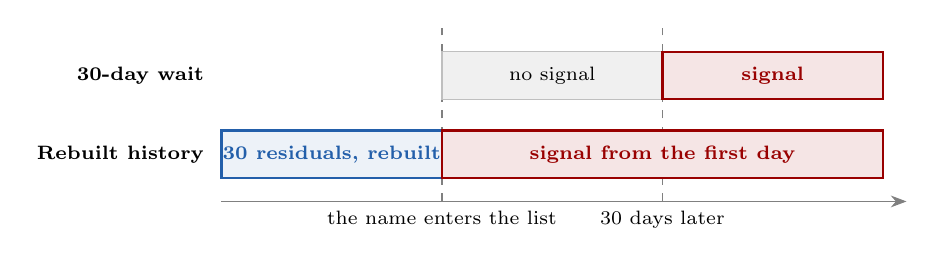
\begin{tikzpicture}[x=1mm,y=1mm,font=\scriptsize]
  % time runs to the right; the name enters the list at x = 50, and 30 days later is x = 78
  \draw[-{Stealth[length=2mm]},draw=gray] (22,0) -- (109,0);
  \draw[draw=gray,dashed] (50,0) -- (50,22);
  \draw[draw=gray,dashed] (78,0) -- (78,22);
  \node[below] at (50,0) {the name enters the list};
  \node[below] at (78,0) {30 days later};
  % 30-day wait
  \node[anchor=east,font=\scriptsize\bfseries] at (21,16) {30-day wait};
  \draw[draw=gray!50,fill=gray!12] (50,13) rectangle (78,19);
  \node at (64,16) {no signal};
  \draw[draw=SBred,fill=SBred!10,thick] (78,13) rectangle (106,19);
  \node[text=SBred,font=\scriptsize\bfseries] at (92,16) {signal};
  % rebuilt history
  \node[anchor=east,font=\scriptsize\bfseries] at (21,6) {Rebuilt history};
  \draw[draw=AttentionBlue,fill=AttentionBlue!8,thick] (22,3) rectangle (50,9);
  \node[text=AttentionBlue,font=\scriptsize\bfseries] at (36,6) {30 residuals, rebuilt};
  \draw[draw=SBred,fill=SBred!10,thick] (50,3) rectangle (106,9);
  \node[text=SBred,font=\scriptsize\bfseries] at (78,6) {signal from the first day};
\end{tikzpicture}
\end{center}

\textbf{30-day wait:} a new name gets no LongConv signal for its first 30 days on the list.
It is still held, but only inside the hedges of other stocks.

\smallskip
\textbf{Rebuilt history:} on day $t$, recompute every member's 30 residuals over today's list,
also for the days before the name entered.

\begin{itemize}
\item No look-ahead: today's list was fixed at the previous month-end.
\item 1 March 2000: 435 names have a signal under the wait; rebuilt, 494.
\end{itemize}
\claim{Stock-days with a signal: $96.2\%\rightarrow99.8\%$.}
\end{frame}

\begin{frame}{Choice 2: Plain List, or Buffered List?}
\small
\textbf{Plain list}, as in the paper: the 500 largest each month. A name near rank 500 goes in and out.

\smallskip
\textbf{Buffered list:} the 500 largest, plus last month's members that still rank within 600.
\begin{center}
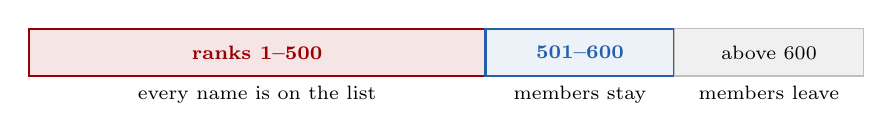
\begin{tikzpicture}[x=1mm,y=1mm,font=\scriptsize]
  \draw[draw=SBred,fill=SBred!10,thick] (0,0) rectangle (58,6);
  \node[text=SBred,font=\scriptsize\bfseries] at (29,3) {ranks 1--500};
  \draw[draw=AttentionBlue,fill=AttentionBlue!8,thick] (58,0) rectangle (82,6);
  \node[text=AttentionBlue,font=\scriptsize\bfseries] at (70,3) {501--600};
  \draw[draw=gray!50,fill=gray!12] (82,0) rectangle (106,6);
  \node at (94,3) {above 600};
  \node[below] at (29,0) {every name is on the list};
  \node[below] at (70,0) {members stay};
  \node[below] at (94,0) {members leave};
\end{tikzpicture}
\end{center}
\begin{center}
\begin{tabular}{@{}lrr@{}}
\toprule
1998--2021 & Plain & Buffered\\
\midrule
Names on the list, per day & $499$ & $543$\\
New names, per month & $14.9$ & $7.0$\\
Stock-days without a signal under the 30-day wait & $3.9\%$ & $1.8\%$\\
\bottomrule
\end{tabular}
\end{center}
\claim{Half as many new names: fewer forced trades and missing histories.}
\end{frame}

\begin{frame}{Four Datasets}
Two choices, two options each:
\begin{center}
\begin{tabular}{@{}cllrr@{}}
\toprule
Dataset & List & 30-day history & Names per day & No signal\\
\midrule
A & Plain & 30-day wait & $499$ & $3.9\%$\\
B & Plain & Rebuilt & $499$ & $0.2\%$\\
C & Buffered & 30-day wait & $543$ & $1.8\%$\\
D & Buffered & Rebuilt & $543$ & $0.2\%$\\
\bottomrule
\end{tabular}
\end{center}
{\footnotesize No signal: share of member stock-days in 1998--2021 without a LongConv signal.\par}

\medskip
\textbf{One setting for all four:}
\begin{itemize}
\item $K=30$ factors, $\lambda_{\rm ridge}=10^{-4}$, 30 epochs, costs of 5 bp and 1 bp.
\item The same 39 ranks, with no filling.
\item Three seeds, traded as one ensemble.
\end{itemize}
\end{frame}

\begin{frame}{Results: Net Sharpe of the Four Datasets}
\begin{center}
\begin{tabular}{@{}llrr@{}}
\toprule
 & & \multicolumn{2}{c}{Net Sharpe}\\
\cmidrule(l){3-4}
Dataset & List, 30-day history & 1998--2021 & 2022--2025\\
\midrule
A & Plain, 30-day wait & $1.56$ & $-0.23$\\
B & Plain, rebuilt & $1.62$ & $-0.15$\\
C & Buffered, 30-day wait & $1.61$ & $-0.28$\\
\textbf{D} & \textbf{Buffered, rebuilt} & $\mathbf{1.70}$ & $\boldsymbol{-}\mathbf{0.18}$\\
\midrule
Paper, $K=30$ & 500 largest & $2.28$ & --\\
\bottomrule
\end{tabular}
\end{center}
\begin{itemize}
\item 1998--2021 is the paper's sample; 2022--2025 is our extension.
\item Annualized, on excess returns after costs: 5 bp per traded unit, 1 bp on short exposure.
\end{itemize}
\src{Ours: one ensemble book from three seeds, $K=30$. Paper: Table 2, single models (its Table 3 states averages over seeds).}
\end{frame}

\begin{frame}{What the Comparison Shows}
\begin{itemize}
\item Each choice adds a little: less than $0.1$ in 1998--2021.
\item D beats A by $0.13$, with a 95\% interval of $-0.06$ to $+0.34$.
\item The validation years 1996--1997 agree: D first, A last.
\item In 2022--2025 no dataset earns its costs.
\item The gap to the paper remains: $1.70$ against $2.28$.
\end{itemize}
\claim{We will use D: the buffered list with rebuilt history.}
\end{frame}

% ============================================================================
\section{The best fixed setting}
\sectiontitlepage

\begin{frame}{The Scan: The Best Fixed Setting for D}
D is our dataset: buffered list, rebuilt 30-day history.
Next we look for the best \emph{fixed} setting of four levers, for every $K=1,3,5,8,15,30,100$:
\begin{center}
\small
\begin{tabular}{@{}lll@{}}
\toprule
Lever & When & Values scanned\\
\midrule
Training cost & In training & 2.5, 5, 7.5, 10 bp\\
Ridge $\lambda_{\rm ridge}$ & In training & 5 values, $10^{-5}$ to $10^{-3}$\\
Epochs & In training & 20, 30, 50, 80\\
Band width $\delta$ & After training & 9 values, $0$ to $0.32\%$ of the book\\
\bottomrule
\end{tabular}
\end{center}
\begin{itemize}
\item Fixed: chosen once, then kept for every year from 1998 to 2025. The models are still retrained every year.
\item Best: the highest net Sharpe on 1996--1997, the last two years of the first training window, as in the paper.
\item The ensemble is always on: three seeds, and we can add more.
\end{itemize}
\claim{One setting for each $K$, chosen before the test years 1998--2025.}
\end{frame}

\begin{frame}{What We Scanned}
\claim{1. The validation years 1996--1997, for every $K$}\par
32 training settings $\times$ 9 band widths: 288 fixed settings for each $K$.
The one with the best net Sharpe of the ensemble with the band is that $K$'s setting.

\medskip
\claim{2. The test years 1998--2025, for every $K$}\par
Each $K$ trained at its own setting: three seeds, retrained every year.

\medskip
\claim{3. The grid on 1998--2025, for $K=8$, $30$ and $100$}\par
28 training settings $\times$ 9 band widths at $K=8$ and $30$; at $K=100$, 3~costs $\times$ 3~ridges at 30 epochs.
To see how each lever acts: nothing is chosen from it.

\medskip
{\small The 32 training settings: 4 costs $\times$ 5 ridges at 30 epochs, plus 20, 50 and 80 epochs
at $\lambda_{\rm ridge}=10^{-4}$ for each cost. The grid on 1998--2025 leaves out 80 epochs.\par}
\end{frame}

\begin{frame}{Results of the Scan}
\small
Net Sharpe on D: each $K$ at its best fixed setting, chosen on 1996--1997.
\begin{center}
\setlength{\tabcolsep}{4pt}
\begin{tabular}{@{}lllrrr@{}}
\toprule
 & \multicolumn{2}{c}{Fixed setting} & Paper & \multicolumn{2}{c}{Ours}\\
\cmidrule(lr){2-3}\cmidrule(l){5-6}
 & Cost, $\lambda_{\rm ridge}$, epochs & Band & 1998--2021 & 1998--2021 & 2022--2025\\
\midrule
$K=1$ & 10 bp, $10^{-4}$, 80 & $0.12\%$ & $1.68$ & $1.66$ & $-0.23$\\
$K=3$ & 7.5 bp, $10^{-4}$, 80 & $0.12\%$ & $1.69$ & $1.54$ & $-0.10$\\
$K=5$ & 5 bp, $10^{-4}$, 80 & $0.08\%$ & $1.58$ & $1.46$ & $-0.97$\\
$K=8$ & 5 bp, $10^{-4}$, 80 & $0.04\%$ & $1.94$ & $1.29$ & $-1.17$\\
$K=15$ & 2.5 bp, $10^{-4}$, 50 & $0.08\%$ & $2.25$ & $1.42$ & $-1.45$\\
$K=30$ & 5 bp, $3\cdot10^{-4}$, 30 & $0.04\%$ & $2.28$ & $2.09$ & $-0.18$\\
$K=100$ & 7.5 bp, $3\cdot10^{-4}$, 30 & $0.02\%$ & $2.19$ & $2.08$ & $+0.25$\\
\bottomrule
\end{tabular}
\end{center}
\begin{itemize}
\item $K=1$ and $3$: near the paper's net Sharpe, at 1.5 to 2 times its volatility.
\item $K=5$ to $15$: the chosen settings train long and trade too much.
\end{itemize}
\claim{$K=30$ and $K=100$ come within $0.2$ of the paper.}
\src{Ours: one ensemble book from three seeds, through the band. Paper: Table 2, single models.}
\end{frame}

\begin{frame}{What the Whole Grid Shows}
\small
Ensemble with the band; at $K=100$ the grid is 3~costs $\times$ 3~ridges:
\begin{center}
\setlength{\tabcolsep}{4pt}
\begin{tabular}{@{}lrrrrr@{}}
\toprule
 & Paper & \multicolumn{2}{c}{Chosen on 1996--1997} & \multicolumn{2}{c}{Chosen on 1998--2021}\\
\cmidrule(lr){3-4}\cmidrule(l){5-6}
Net Sharpe & 1998--2021 & 1998--2021 & 2022--2025 & 1998--2021 & 2022--2025\\
\midrule
$K=8$ & $1.94$ & $1.29$ & $-1.17$ & $2.22$ & $-0.40$\\
$K=30$ & $2.28$ & $2.09$ & $-0.18$ & $2.28$ & $+0.13$\\
$K=100$ & $2.19$ & $2.08$ & $+0.25$ & $2.26$ & $+0.35$\\
\bottomrule
\end{tabular}
\end{center}
Chosen on 1998--2021, all at 30 epochs: 5 bp, $\lambda_{\rm ridge}=10^{-4}$, band $0.12\%$ at $K=8$ and $30$;
10 bp, $3\cdot10^{-4}$, band $0.04\%$ at $K=100$.
An upper bound: scored on the years it is chosen on. 2022--2025 is out of sample for both.

At $K=8$, 1996--1997 rewards long training; 1998--2021 does not:
\begin{center}
\begin{tabular}{@{}lrrrr@{}}
\toprule
Epochs, at 5 bp and $\lambda_{\rm ridge}=10^{-4}$ & 20 & 30 & 50 & 80\\
\midrule
Net Sharpe, 1996--1997 & $8.20$ & $9.15$ & $9.88$ & $\mathbf{10.10}$\\
Net Sharpe, 1998--2021 & $2.02$ & $\mathbf{2.12}$ & $1.88$ & $1.29$\\
\bottomrule
\end{tabular}
\end{center}
\claim{The grid reaches the paper; choosing on 1996--1997 misses it at $K=8$.}
\src{The band is chosen with the rest of the setting: on 1996--1997, or on 1998--2021 in the last two columns.}
\end{frame}

% ============================================================================
\section{Conclusions and next steps}
\sectiontitlepage

\begin{frame}{Conclusions and Next Steps}
\small
\textbf{What we built:}
\begin{itemize}
\item The model: attention factors and LongConv, trained on the annualized net Sharpe.
\item The data: 39 characteristics from WRDS, checked against the Chen--Pelger--Zhu panel, with no filling.
\item The universe: the buffered list with rebuilt 30-day history.
\end{itemize}
\textbf{What we get so far}, net Sharpe in 1998--2021 (2022--2025):
\begin{itemize}
\item D, $K=30$, seed ensemble: $1.70$ ($-0.18$); the paper: $2.28$.
\item Best fixed setting, with the band: $2.09$ ($-0.18$) at $K=30$, $2.08$ ($+0.25$) at $K=100$.
\end{itemize}
\textbf{Next:}
\begin{itemize}
\item $K=5$ to $15$: a fixed setting that holds beyond 1996--1997.
\item Explore the role of $\lambda_{\rm Var}$: annualizing set it, in effect, to $6.3$.
\item More seeds in the ensemble.
\item Where the remaining gap to the paper comes from.
\end{itemize}
\end{frame}

\begin{frame}{References}
\scriptsize
\begin{itemize}
\item Epstein, Wang, Choi and Pelger (2025). \emph{Attention Factors for Statistical Arbitrage}. \href{https://doi.org/10.1145/3768292.3770398}{ICAIF paper}.
\item Chen, Pelger and Zhu. \emph{Deep Learning in Asset Pricing}. \href{https://arxiv.org/abs/1904.00745}{Author manuscript and Internet Appendix}; replication panel of characteristics.
\item Guijarro-Ordonez, Pelger and Zanotti. \emph{Deep Learning Statistical Arbitrage}. \href{https://arxiv.org/abs/2106.04028}{Author manuscript}.
\item Fu et al. (2023). \emph{Simple Hardware-Efficient Long Convolutions for Sequence Modeling}. \href{https://proceedings.mlr.press/v202/fu23a.html}{ICML}.
\item Avellaneda and Lee (2010). \emph{Statistical Arbitrage in the US Equities Market}.
\item WRDS: CRSP daily and monthly stock files, Compustat annual fundamentals, CRSP--Compustat links, Fama--French factors.
\end{itemize}
\end{frame}

% --- Closing ----------------------------------------------------------------

\begin{frame}{Thanks!}
\claim{Any questions?}
\end{frame}

% --- Backup slides (after the closing frame, as in Phase I) -----------------

\begin{frame}{Settings of the Four-Dataset Runs}
\small
\begin{tabular}{@{}lr@{}}\toprule
Setting & Value\\\midrule
Factors $K$ & 30\\
Attention embedding & 32\\
LongConv hidden channels / layers & 32 / 1\\
Residual lookback & 30 trading days\\
Training window / refit & 8 years / annual\\
Epochs / learning rate / optimizer & 30 / 0.003 / AdamW\\
Dropout / LongConv weight decay & 0.1 / 0.05\\
Explained-variance coefficient & 100\\
Ridge $\lambda_{\rm ridge}$ & $10^{-4}$\\
Kernel squash threshold & 0.001\\
Costs: trading / shorting & 5 bp / 1 bp\\
Seeds & 0, 1, 2, as one ensemble\\
Validation / test / extension & 1996--1997 / 1998--2021 / 2022--2025\\\bottomrule
\end{tabular}\par
\end{frame}

% The formulas of the 39 characteristics and the risk-free rate, as built (the user's request, 2026-11-15).
% Sources: analysis/characteristics/market.md section 3, accounting.md section 3, training_data.md section 4.
\newcommand{\ch}[1]{\texttt{#1}}            % a characteristic
\newcommand{\cz}[1]{\mathrm{#1}^{*}}        % a Compustat item that counts as 0 when missing

\begin{frame}{Formulas: Daily Characteristics and $r_f$}
\small
Row $t$ holds what is known at the close of day $t-1$. $R_{i,d}$ is the return of stock $i$ on day $d$,
and $V_{i,d}$ its shares traded. All five days must have data.
\begin{center}
\renewcommand{\arraystretch}{1.7}
\begin{tabular}{@{}ll@{}}
\toprule
\ch{Ret\_D1} & $R_{i,t-1}$\\
\ch{Ret\_W1} & $\prod_{d=t-5}^{t-1}(1+R_{i,d})-1$\\
\ch{STD\_W1} & $\Big(\frac14\sum_{d=t-5}^{t-1}\big(R_{i,d}-\bar R_i\big)^2\Big)^{1/2}$,
               \quad $\bar R_i=\frac15\sum_{d=t-5}^{t-1}R_{i,d}$\\
\ch{Vol} & $\sum_{d=t-5}^{t-1}V_{i,d}$\\
\midrule
Risk-free rate & $r_{f,d}=(1+r_{f,m})^{1/n_m}-1$, the same for every stock\\
\bottomrule
\end{tabular}
\end{center}
$r_{f,m}$ is the Fama--French rate of day $d$'s month $m$, and $n_m$ the number of trading days
that month was scheduled to have. Row $t$ holds $r_{f,t-1}$.

\medskip
A stock's 79 inputs: its 39 ranks, the 39 cross-sectional medians, and $r_{f,t-1}$.
\end{frame}

\begin{frame}{Formulas: Monthly, Past Returns}
\small
$f$ is the formation month, the month before the holding month. $R_{i,m}$ is the return of month $m$,
as in CRSP's legacy monthly file, where a dividend is not reinvested within the month:
\[
R_{i,m}=\prod_{d\in m}(1+x_{i,d})-1+\sum_{d\in m}y_{i,d}\prod_{s\in m,\ s<d}(1+x_{i,s}),
\]
with $x_{i,d}$ the day's price return and $y_{i,d}$ its dividend yield.
\begin{center}
\renewcommand{\arraystretch}{1.6}
\begin{tabular}{@{}ll@{}}
\toprule
\ch{ST\_Rev} & $R_{i,f}$\\
\ch{r2\_1} & $R_{i,f-1}$\\
\ch{r12\_2} & $\prod_{m=f-11}^{f-1}(1+R_{i,m})-1$\\
\ch{r12\_7} & $\prod_{m=f-11}^{f-6}(1+R_{i,m})-1$\\
\ch{r36\_13} & $\prod_{m=f-35}^{f-12}(1+R_{i,m})-1$\\
\bottomrule
\end{tabular}
\end{center}
Every month of a window must have a return.
\end{frame}

\begin{frame}{Formulas: Monthly, Trading Frictions (1/2)}
\small
Sums run over the trading days $d$ of the months named, and $n$ is their number.
\begin{center}
\renewcommand{\arraystretch}{1.6}
\begin{tabular}{@{}ll@{}}
\toprule
\ch{LME} & $P_{i,f}\,S_{i,f}$, in \$ million\\
\ch{LTurnover} & $\operatorname{round}(V_{i,f}/100)\,\big/\,(S_{i,f}/1000)$\\
\ch{Rel2High} & $\tilde P_{i,f}\,\big/\max_{d\in f-11,\dots,f}\tilde P_{i,d}$\\
\ch{Spread} & $\frac1n\sum_{d\in f}\frac{H_{i,d}-L_{i,d}}{(H_{i,d}+L_{i,d})/2}$\\
\ch{Variance} & $\frac1{n-1}\sum_{d\in f-1,\,f}\big(R_{i,d}-\bar R_i\big)^2$\\
\bottomrule
\end{tabular}
\end{center}
\begin{itemize}
\item $P_{i,f}$: last price of month $f$. $S_{i,f}$: shares outstanding at its end. $V_{i,f}$: shares traded in it.
\item $\tilde P_{i,d}$: split-adjusted close. $H$, $L$: the day's high and low; ask and bid on a day without a trade.
\item LTurnover keeps the units of CRSP's legacy file: volume in hundreds, shares in thousands.
\end{itemize}
\end{frame}

\begin{frame}{Formulas: Monthly, Trading Frictions (2/2)}
\small
\setlength{\abovedisplayskip}{3pt}
\setlength{\belowdisplayskip}{3pt}
\ch{Resid\_Var}$_i=\frac{1}{n-1}\sum_d\hat e_{i,d}^{\,2}$, from a fit on the $n$ days of months $f-1$ and $f$, at least 20:
\[
R_{i,d}-r_{f,d}=a_i+b_i\,\mathrm{MKT}_d+c_i\,\mathrm{SMB}_d+g_i\,\mathrm{HML}_d+e_{i,d}.
\]
\ch{SUV}$_i=\frac{1}{n_f}\sum_{d\in f}\big(V_{i,d}-\hat V_{i,d}\big)/\hat s_i$ over the $n_f$ days of $f$,
from a fit on the $n_0$ days of months $f-2$ and $f-1$, at least 5:
\[
V_{i,d}=a_i+b_i\,(R_{i,d})^{+}+c_i\,(-R_{i,d})^{+}+u_{i,d},
\qquad
\hat s_i^{\,2}=\frac{1}{n_0-1}\sum_d\hat u_{i,d}^{\,2}.
\]
\ch{Beta} $=\rho_i\,\sigma_i/\sigma_M$, as in Frazzini and Pedersen:
\begin{itemize}
\item $\sigma_i$: standard deviation of $\ln(1+R_{i,d})$ over months $f-11,\dots,f$, at least 120 days.
\item $\sigma_M$: standard deviation of $\ln(1+\mathrm{MKT}_d)$ over every trading day of those months.
\item $\rho_i$: correlation over months $f-59,\dots,f$ of sums over 3 consecutive observations of
      $\ln(1+R_{i,d}-r_{f,d})$ and of $\ln(1+\mathrm{MKT}_d)$ on the same days, at least 750 sums.
\end{itemize}
\src{MKT, SMB, HML: the Fama--French daily factors; MKT is the market's return in excess of $r_f$. $V_{i,d}$: shares traded. $x^{+}=\max(x,0)$.}
\end{frame}

\begin{frame}{Formulas: Yearly, Total Assets and Value}
\small
\setlength{\abovedisplayskip}{3pt}
\setlength{\belowdisplayskip}{3pt}
Compustat items of the fiscal year in use, $\tau$; a subscript $\tau-1$ marks the year before.
ME is the stock's market cap at the end of December of year $\tau$.
Items marked $^{*}$ count as $0$ when missing; the others are essential.
\[
\mathrm{BE}=\mathrm{SEQ}-\cz{PS}+\cz{TXDITC},
\quad
\mathrm{PS}=\mathrm{PSTKRV},\ \text{else}\ \mathrm{PSTKL},\ \text{else}\ \mathrm{PSTK}.
\]
\begin{center}
\begin{tabular}{@{}ll@{}}
\toprule
\ch{AT} & $\mathrm{AT}$\\
\ch{A2ME} & $\mathrm{AT}/\mathrm{ME}$\\
\ch{BEME} & $\mathrm{BE}/\mathrm{ME}$\\
\ch{C} & $\mathrm{CHE}/\mathrm{AT}$\\
\ch{CF} & $(\mathrm{NI}+\mathrm{DP}-\cz{WCAPCH}-\cz{CAPX})/\mathrm{BE}$\\
\ch{CF2P} & $(\mathrm{IB}+\mathrm{DP}+\cz{TXDB})/\mathrm{ME}$\\
\ch{Q} & $(\mathrm{AT}+\mathrm{CSHO}\times\mathrm{PRCC\_F}-\mathrm{CEQ}-\cz{TXDB})/\mathrm{AT}$\\
\ch{Lev} & $(\cz{DLTT}+\cz{DLC})/(\cz{DLTT}+\cz{DLC}+\mathrm{SEQ})$\\
\ch{E2P} & $\mathrm{IB}/\mathrm{ME}$\\
\bottomrule
\end{tabular}
\end{center}
\src{TXDITC is added only up to fiscal year 1992. SEQ is never missing in our universe.
AT total assets; SEQ shareholders' equity; CEQ common equity; PSTKRV, PSTKL, PSTK preferred stock at redemption, liquidating and par value;
TXDITC deferred taxes and investment tax credit; CHE cash and short-term investments; NI net income; DP depreciation and amortization;
WCAPCH change in working capital; CAPX capital expenditures; IB income before extraordinary items; TXDB deferred taxes;
CSHO shares outstanding; PRCC\_F price at the fiscal year-end; DLTT long-term debt; DLC debt in current liabilities.}
\end{frame}

\begin{frame}{Formulas: Yearly, Profitability}
\small
Notation as on the previous slide. Net operating assets:
\begingroup\footnotesize
\[
\mathrm{NOA}^{\rm raw}=(\mathrm{AT}-\mathrm{CHE}-\cz{IVAO})-(\mathrm{AT}-\cz{DLC}-\cz{DLTT}-\cz{MIB}-\cz{PSTK}-\mathrm{CEQ}).
\]
\endgroup
\begin{center}
\renewcommand{\arraystretch}{1.4}
\begin{tabular}{@{}ll@{}}
\toprule
\ch{PROF} & $(\mathrm{REVT}-\mathrm{COGS})/\mathrm{BE}$\\
\ch{CTO} & $\mathrm{SALE}/\mathrm{AT}_{\tau-1}$\\
\ch{FC2Y} & $(\mathrm{XSGA}+\cz{XRD}+\cz{XAD})/\mathrm{SALE}$\\
\ch{OP} & $(\mathrm{REVT}-\mathrm{COGS}-\cz{TIE}-\mathrm{XSGA})/\mathrm{BE}$\\
\ch{PM} & $\mathrm{OIADP}/\mathrm{SALE}$\\
\ch{RNA} & $\mathrm{OIADP}/\mathrm{NOA}^{\rm raw}_{\tau-1}$\\
\ch{D2A} & $\mathrm{DP}/\mathrm{AT}$\\
\bottomrule
\end{tabular}
\end{center}
\src{REVT revenue; COGS cost of goods sold; SALE net sales; XSGA selling, general and administrative expense;
XRD research and development expense; XAD advertising expense; TIE total interest expense, reported by financial firms;
OIADP operating income after depreciation; IVAO other investments and advances; MIB minority interest.}
\end{frame}

\begin{frame}{Formulas: Yearly, Investment and Intangibles}
\small
Notation as before; $\Delta$ is the change from $\tau-1$ to $\tau$. Working capital:
\[
\mathrm{WC}=\mathrm{ACT}-\mathrm{CHE}-\mathrm{LCT}-\cz{DLC}-\cz{TXP}-\mathrm{DP}.
\]
\begin{center}
\renewcommand{\arraystretch}{1.4}
\begin{tabular}{@{}ll@{}}
\toprule
\ch{Investment} & $\mathrm{AT}/\mathrm{AT}_{\tau-1}-1$\\
\ch{NOA} & $\mathrm{NOA}^{\rm raw}/\mathrm{AT}_{\tau-1}$\\
\ch{DPI2A} & $(\Delta\mathrm{PPEGT}+\Delta\cz{INVT})/\mathrm{AT}_{\tau-1}$\\
\midrule
\ch{OA} & $(\mathrm{WC}-\mathrm{WC}_{\tau-1})/\mathrm{AT}_{\tau-1}$\\
\ch{OL} & $(\mathrm{COGS}+\mathrm{XSGA})/\mathrm{AT}$\\
\ch{PCM} & $(\mathrm{SALE}-\mathrm{COGS})/\mathrm{SALE}$\\
\bottomrule
\end{tabular}
\end{center}
\src{ACT current assets; LCT current liabilities; TXP income taxes payable; PPEGT gross property, plant and equipment; INVT inventories.}
\end{frame}

\begin{frame}{Where the Panel Overrides the Written Definition}
\small
\begin{tabular}{@{}l>{\raggedright\arraybackslash}p{.76\textwidth}@{}}\toprule
Name & What reproduces the panel\\\midrule
\texttt{r2\_1} & Return of month $t-2$; \texttt{ST\_Rev} is month $t-1$\\[1mm]
\texttt{Spread} & Mean daily high--low range, not a quoted spread\\[1mm]
\texttt{Q} & Compustat shares times year-end price, not CRSP's cap\\[1mm]
\texttt{Beta} & Log returns; a five-year correlation of three-day sums times a one-year volatility ratio\\[1mm]
\texttt{OA} & Change of the whole working-capital bracket, depreciation included, over lagged assets\\[1mm]
Book equity & Deferred taxes are added only up to fiscal year 1992\\\bottomrule
\end{tabular}\par
\medskip
\textbf{Two departures from the panel, to avoid look-ahead:}
\begin{itemize}
\item Annual accounts enter 4 months after the fiscal year-end, 6 for ADRs and foreign issuers.
\item Residual variance and beta use today's Fama--French factor file.
\end{itemize}
\end{frame}

\begin{frame}{Share of Stock-Days at Rank $0$}
\small
With no filling, a characteristic without a value sits at rank $0$:
\begin{center}
\begin{tabular}{@{}lrlr@{}}
\toprule
Characteristic & No value & Characteristic & No value\\
\midrule
\texttt{FC2Y} & $22.7\%$ & \texttt{CF2P} & $7.2\%$\\
\texttt{OP}, \texttt{OL} & $22.6\%$ & \texttt{CF}, \texttt{D2A} & $5.7\%$\\
\texttt{OA} & $20.8\%$ & \texttt{Beta} & $5.3\%$\\
\texttt{DPI2A} & $11.0\%$ & \texttt{r36\_13} & $5.2\%$\\
\bottomrule
\end{tabular}
\end{center}
\begin{itemize}
\item All other characteristics: under $2\%$.
\item Most of the accounting gaps are financial firms.
\item A missing input counts as zero only where the panel shows it and a missing item plausibly
      means none. Missing selling and administrative expenses leave \texttt{FC2Y} empty.
\end{itemize}
\end{frame}

\begin{frame}{Rebuilt History: The Rule in Detail}
On day $t$, every member of today's list gets 30 residuals, all computed over today's list.
\begin{itemize}
\item For a past day $s$: factor baskets from the members' characteristics of day $s-1$,
      residuals from their returns of day $s$.
\item A past day keeps its own day's characteristics: nothing from after $s$ is used.
\item Today's list was fixed at the previous month-end.
\end{itemize}
\textbf{Exception:} no signal until the stock has
\begin{itemize}
\item 30 trading days since its listing, and
\item an annual report that has entered.
\end{itemize}
Such a stock stays in the factor baskets and in the hedges.

\claim{Left without a signal: $0.2\%$ of stock-days.}
\end{frame}

\begin{frame}{Dataset D Against the Paper}
1998--2021, $K=30$, annualized:
\begin{center}
\begin{tabular}{@{}lrrrrrr@{}}
\toprule
 & SR & $\mu$ & $\sigma$ & $\mathrm{SR}_{\rm net}$ & $\mu_{\rm net}$ & Turnover\\
\midrule
Paper & $3.97$ & $16.66$ & $4.20$ & $2.28$ & $9.52$ & $0.47^{*}$\\
D, ensemble & $3.89$ & $15.90$ & $4.08$ & $1.70$ & $6.89$ & $0.62$\\
\bottomrule
\end{tabular}
\end{center}
\begin{itemize}
\item Before costs the two are close.
\item After costs we fall short: we trade $0.62$ of the book a day.
\end{itemize}
\src{$\mu$ and $\sigma$ in percent a year; turnover per day. $^{*}$The paper does not report turnover: $0.47$ is implied by its costs if half of the book is short.}
\end{frame}

\end{document}
